\section{The algorithm}\label{sec:the-algorithm}
Suppose an unsorted database containing $N$ items arranged in a completely random order. In order to find a specific item with a probability of $\frac{1}{2}$, any classical algorithm (whether deterministic or probabilistic) will need to look at a minimum of $\frac{N}{2}$ items. Quantum mechanical systems can be in a superposition of states and simultaneously examine multiple names. By properly adjusting the phases of various operations, successful computations reinforce each other while others interfere randomly. As a result, the desired item can be obtained in only $\mathcal{O}(\sqrt{n})$ steps.

Thus in the search problem, it is possible to find the object without examining all of the objects, but just by allowing a certain probability of examining the desired object.
The quantum search algorithm is general as it can be applied far beyond the database search example just described to speed up many, though not all, classical algorithms that use search heuristics.

\subsection{The procedure}
If we want to search through a search space of $N$ elements rather than searching the elements directly we concentrate on the index to those elements, which is a number in the range $0$ to $N-1$. We assume $N=2^n$ in order to be able to store the index in $n$ classical bits. Suppose that the search problem has exactly $M$ solutions, with $1\leq M \leq N$.

The algorithm makes use of a single $n$ qubit register. It begins with the computer in the state $\ket{0}^{\otimes n}$. Then the Hadamard transform discussed in section~\ref{sec:hadamard} is applied in order to initialize the system to the superposition state
\begin{equation}\label{eq:initial-state}
   \ket{\psi} = \frac{1}{\sqrt{N}} \sum_{x=0}^{N-1}\ket{x}
\end{equation}
where $\ket{x}$ is the index register and each index has the same probability amplitude (i.e. $\sqrt{N}$).
The \emph{Grover iteration} of the algorithm may be broken up in four steps:

\begin{enumerate}
  \item Apply the \emph{subroutine} $\hat{U}_\beta$ (we are going to discuss it in section~\ref{sec:subroutine}).
  \item Apply the Hadamard transform $\hat{H}^{\otimes n}$ \label{enum:first-hadamard}
  \item \label{enum:phase-shift} Perform a conditional phase shift on the quantum computer, with every computational basis state except $\ket{0}$ receiving a phase shift of $-1$,
  \begin{equation*}
      \ket{x} \rightarrow -(-1)^{\delta_{x0}} \ket{x}.
  \end{equation*}
  \item Apply the Hadamard transform $\hat{H}^{\otimes n}$ \label{enum:second-hadamard}
\end{enumerate}
Initializing the system is obtained in $\mathcal{O}(\log_2{N})$ steps while steps~\ref{enum:first-hadamard} and~\ref{enum:second-hadamard}, the Hadamard transforms, require $n=\log_2{N}$ operations each. Step~\ref{enum:phase-shift}, the conditional phase shift, may be implemented using $\mathcal{O}(n)$gates. The cost of the subroutine call depends upon the specific application but we can note that the iteration requires only a single subroutine call.


\begin{defn}
We can demonstrate that the unitary operator corresponding to the phase shift in the iteration is $2\ket{0}\bra{0}-\hat{I}$. The combined effect of steps~\ref{enum:first-hadamard},\ref{enum:phase-shift} and~\ref{enum:second-hadamard} is then:
\begin{equation*}
    \hat{H}^{\otimes n} (2\ket{0}\bra{0}-\hat{I}) \hat{H}^{\otimes n} =  2\ket{\psi}\bra{\psi}-\hat{I}
\end{equation*}
with $\ket{\psi}$ being the initial state in~\ref{eq:initial-state}. Those steps may then be written as
\begin{equation*}
    \hat{U}_\psi \equiv 2 \ket{\psi}\bra{\psi} - \hat{I}.
\end{equation*}
\end{defn}
\begin{defn}
We can define the Grover iteration as
\begin{equation}\label{eq:grover-iteration}
G \equiv \hat{U}_\psi\hat{U}_\beta = (2 \ket{\psi}\bra{\psi} - \hat{I}) \hat{U}_\beta
\end{equation}
\end{defn}
\begin{figure}
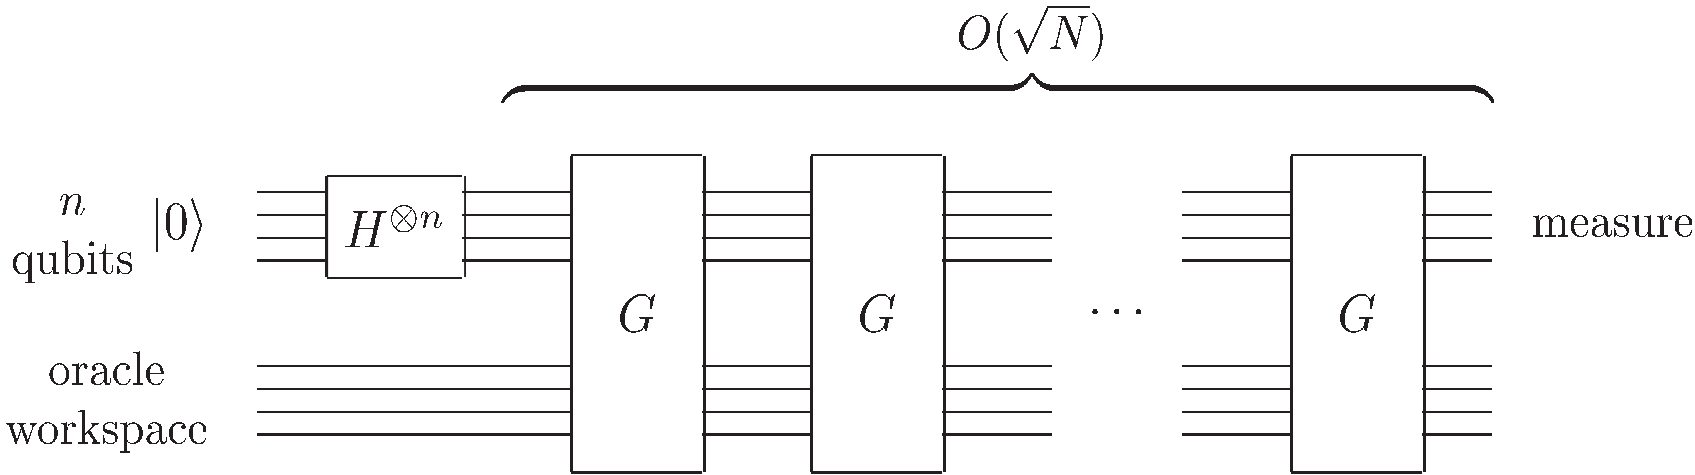
\includegraphics{circuit.png}
\centering
\caption{Circuit for the quantum search algorithm.}
\end{figure}
\begin{figure}
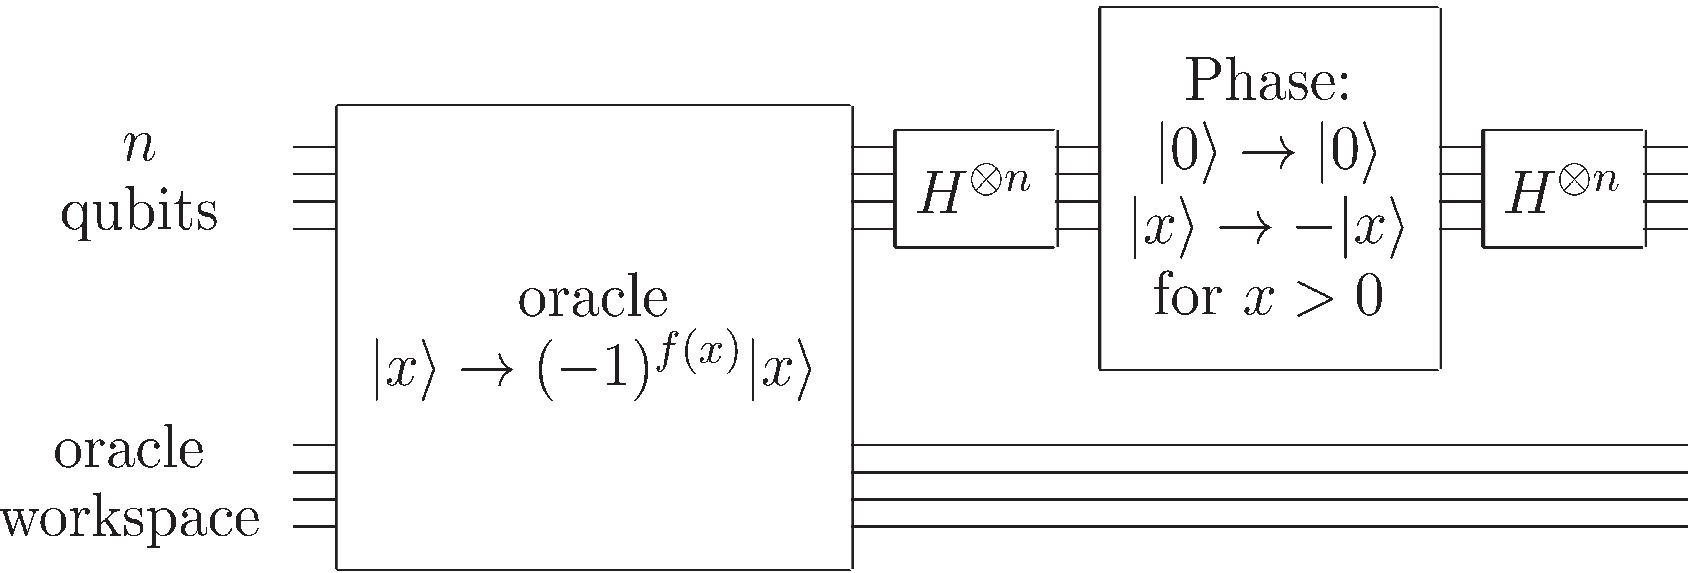
\includegraphics{iteration.png}
\centering
\caption{Iteration $U_\psi U_\beta$}
\end{figure}
Each iteration of this loop increases the amplitude in the desired state by $\mathbb{O}(1/\sqrt{N})$, as a result in $\mathbb{O}(\sqrt{N})$ repetitions of the loop, the amplitude and hence the probability in the desired state reach $\mathbb{O}(1)$.

\subsection{The subroutine}\label{sec:subroutine}
Suppose we are supplied with a black box $f(x)$ whose internal workings are not important with the ability to recognize the solution\footnote{Note that there is a distinction between knowing the solution and being able to recognize the solution. If, for example, we want to find the prime factor of the number $m$ even without not knowing the prime factors we can explicitly construct a subroutine which recognizes a solution when it sees one.}:
\begin{defn}
Let's define the function $f: \{0,1,...,N-1\} \rightarrow \{0,1\}$ as follows
\begin{equation*}
    \begin{cases}
&f(x) = 1   \quad  x=\beta \\
&f(x) = 0   \quad x\neq\beta
\end{cases}
\end{equation*}
with $\beta$ solution to the search problem.
\end{defn}
But furthermore, it is a quantum subroutine, so it can respond to queries that are superpositions of states:
\begin{defn}
The subroutine $\hat{U}_\beta$ is a unitary operator defined by its action on the computational basis
\begin{equation*}
    \ket{x}\ket{q} \xrightarrow{\hat{U}_\beta} \ket{x} \ket{q \oplus f(x)}
\end{equation*}
\end{defn}
where $\ket{x}$ is the index register and $\ket{q}$ is an \emph{oracle qubit}, a single qubit which is flipped if $f(x) = 1$ and is unchanged otherwise.

It is useful to set the oracle qubit initially in the state $\ket{q} = \frac{\ket{0}-\ket{1}}{\sqrt{2}}$ the action of the subroutine is thus\footnote{If $x$ is not a solution, applying the subroutine to $\ket{q}$ leaves the state unchanged. On the other and if $x$ is a solution $\frac{\ket{0 \oplus 1} - \ket{1 \oplus 1}}{\sqrt{2}} = \frac{\ket{1}-\ket{0}}{\sqrt{2}} = - \frac{\ket{0}-\ket{1}}{\sqrt{2}}$. And $\ket{x}$ is not affected by the value of $f(x)$.}:
\begin{equation*}
    \hat{U}_\beta \ket{x} \biggl(\frac{\ket{0}-\ket{1}}{\sqrt{2}}\biggr) = (-1)^{f(x)} \ket{x} \biggl(\frac{\ket{0}-\ket{1}}{\sqrt{2}}\biggr).
\end{equation*}
We can see that the state of the oracle qubit is not changed; it turns out that this remains  $\frac{\ket{0}-\ket{1}}{\sqrt{2}}$ throughout the iteration, and can therefore be omitted:
\begin{equation*}
    \hat{U}_\beta \ket{x} = (-1)^{f(x)} \ket{x}.
\end{equation*}
The subroutine marks the solution by shifting the phase of the solution. Note that in an implementation it would involve a portion of the quantum system sensing the state and then deciding whether or not to rotate the phase. It would to it in a way so that no trace of the state of the system be left after this operation.
\subsection{Example with only one solution}
Until now no assumption were made about the number of solutions $M$, let's now give a complete overview of the algorithm with $M=1$.
\begin{description}
   \item[Inputs] The inputs of the quantum computer are:
    \begin{enumerate}
  \item The subroutine $\hat{U}_\beta$ which perform the transformation $\hat{U}_\beta\ket{x}\ket{q} = \ket{x}\ket{q \oplus f(x)}$, where $f(x) = 0$ for all $0 \leq x \leq 2^n$ except $x_o$.
  \item $n+1$ qubits in the state $\ket{0}$.
\end{enumerate}
   \item[Outputs] $x_0$.
   \item[Runtime] $R = \mathcal{O}(\sqrt{2^n})$ operations\footnote{$R$ has the exact value defined in~\ref{eq:upper-bound} as we will see in section~\ref{sec:performance}}. Succeeds with probability $\mathcal{O}(1)$.
   \item[Procedure] The iteration is the following:
   \begin{enumerate}
  \item $\ket{0}^{\otimes n} \ket{0}$ \label{enum:initial-state}
  \item $\begin{aligned} \rightarrow \frac{1}{\sqrt{2^n}} \sum_{x=0}^{2^n-1}\ket{x} \biggl[\frac{\ket{0}-\ket{1}}{\sqrt{2}}\biggr] \end{aligned}$ \label{enum:hadamard}
  \item $\begin{aligned} \rightarrow \bigl[(2 \ket{\psi}\bra{\psi} - \hat{I})\hat{U}_\beta\bigr]^R \frac{1}{\sqrt{2^n}} \sum_{x=0}^{2^n-1}\ket{x} \biggl[\frac{\ket{0}-\ket{1}}{\sqrt{2}}\biggr] \approx \ket{x_0} \biggl[\frac{\ket{0}-\ket{1}}{\sqrt{2}}\biggr] \end{aligned}$ \label{enum:iteration}
  \item $\rightarrow x_0$ \label{enum:result}
\end{enumerate}
\end{description}

Step~\ref{enum:initial-state} it is simply the initial state. Step~\ref{enum:hadamard} consist of applying $H^{\otimes n}$ to the first $n$ qubits and $H X$ to the last qubit. Step~\ref{enum:iteration} is the Grover iteration defined in~\ref{def:grover-iteration} applied $R$ times and step~\ref{enum:result} is the result.


